\section{Water Bodies} \label{sec:water_bodies}

Water bodies refers here to static water build-ups such as seas, oceans and lakes. The water-flow simulation (see section \ref{sec:rivers_and_streams}) often fails to reproduce these accurately as they are the result of years of water accumulation, groundwater and different soil infiltration rates. Users can place such water bodies by using a \textit{flood-fill}.

Flood-filling uses a single seed point, \textit{P$_{seed}$}, to determine the height, \textit{H$_{level}$}, at which to set the water-level. This seed point then iteratively propagates to all surrounding points which have height \textit{H} equal or lower than \textit{H$_{level}$} using a flood-fill approach. The process continues until there are no more valid destination points or the terrain extremity is reached. When flood-filling is activated, the user specifies the seed point by simply clicking on it with the mouse pointer. The flood-filling algorithm produces water bodies in real-time even for large terrains and large water-bodies. It is possible to undo an unlimited stack of water body placements added with the flood-filling tool (Ctrl+Z). This is deemed important in case the user mistakenly specifies an incorrect seed point. \\

Figure \ref{fig:flood_fill_test} shows that the tool can be used to successfully place water bodies on the terrain.

\begin{figure}
\center
	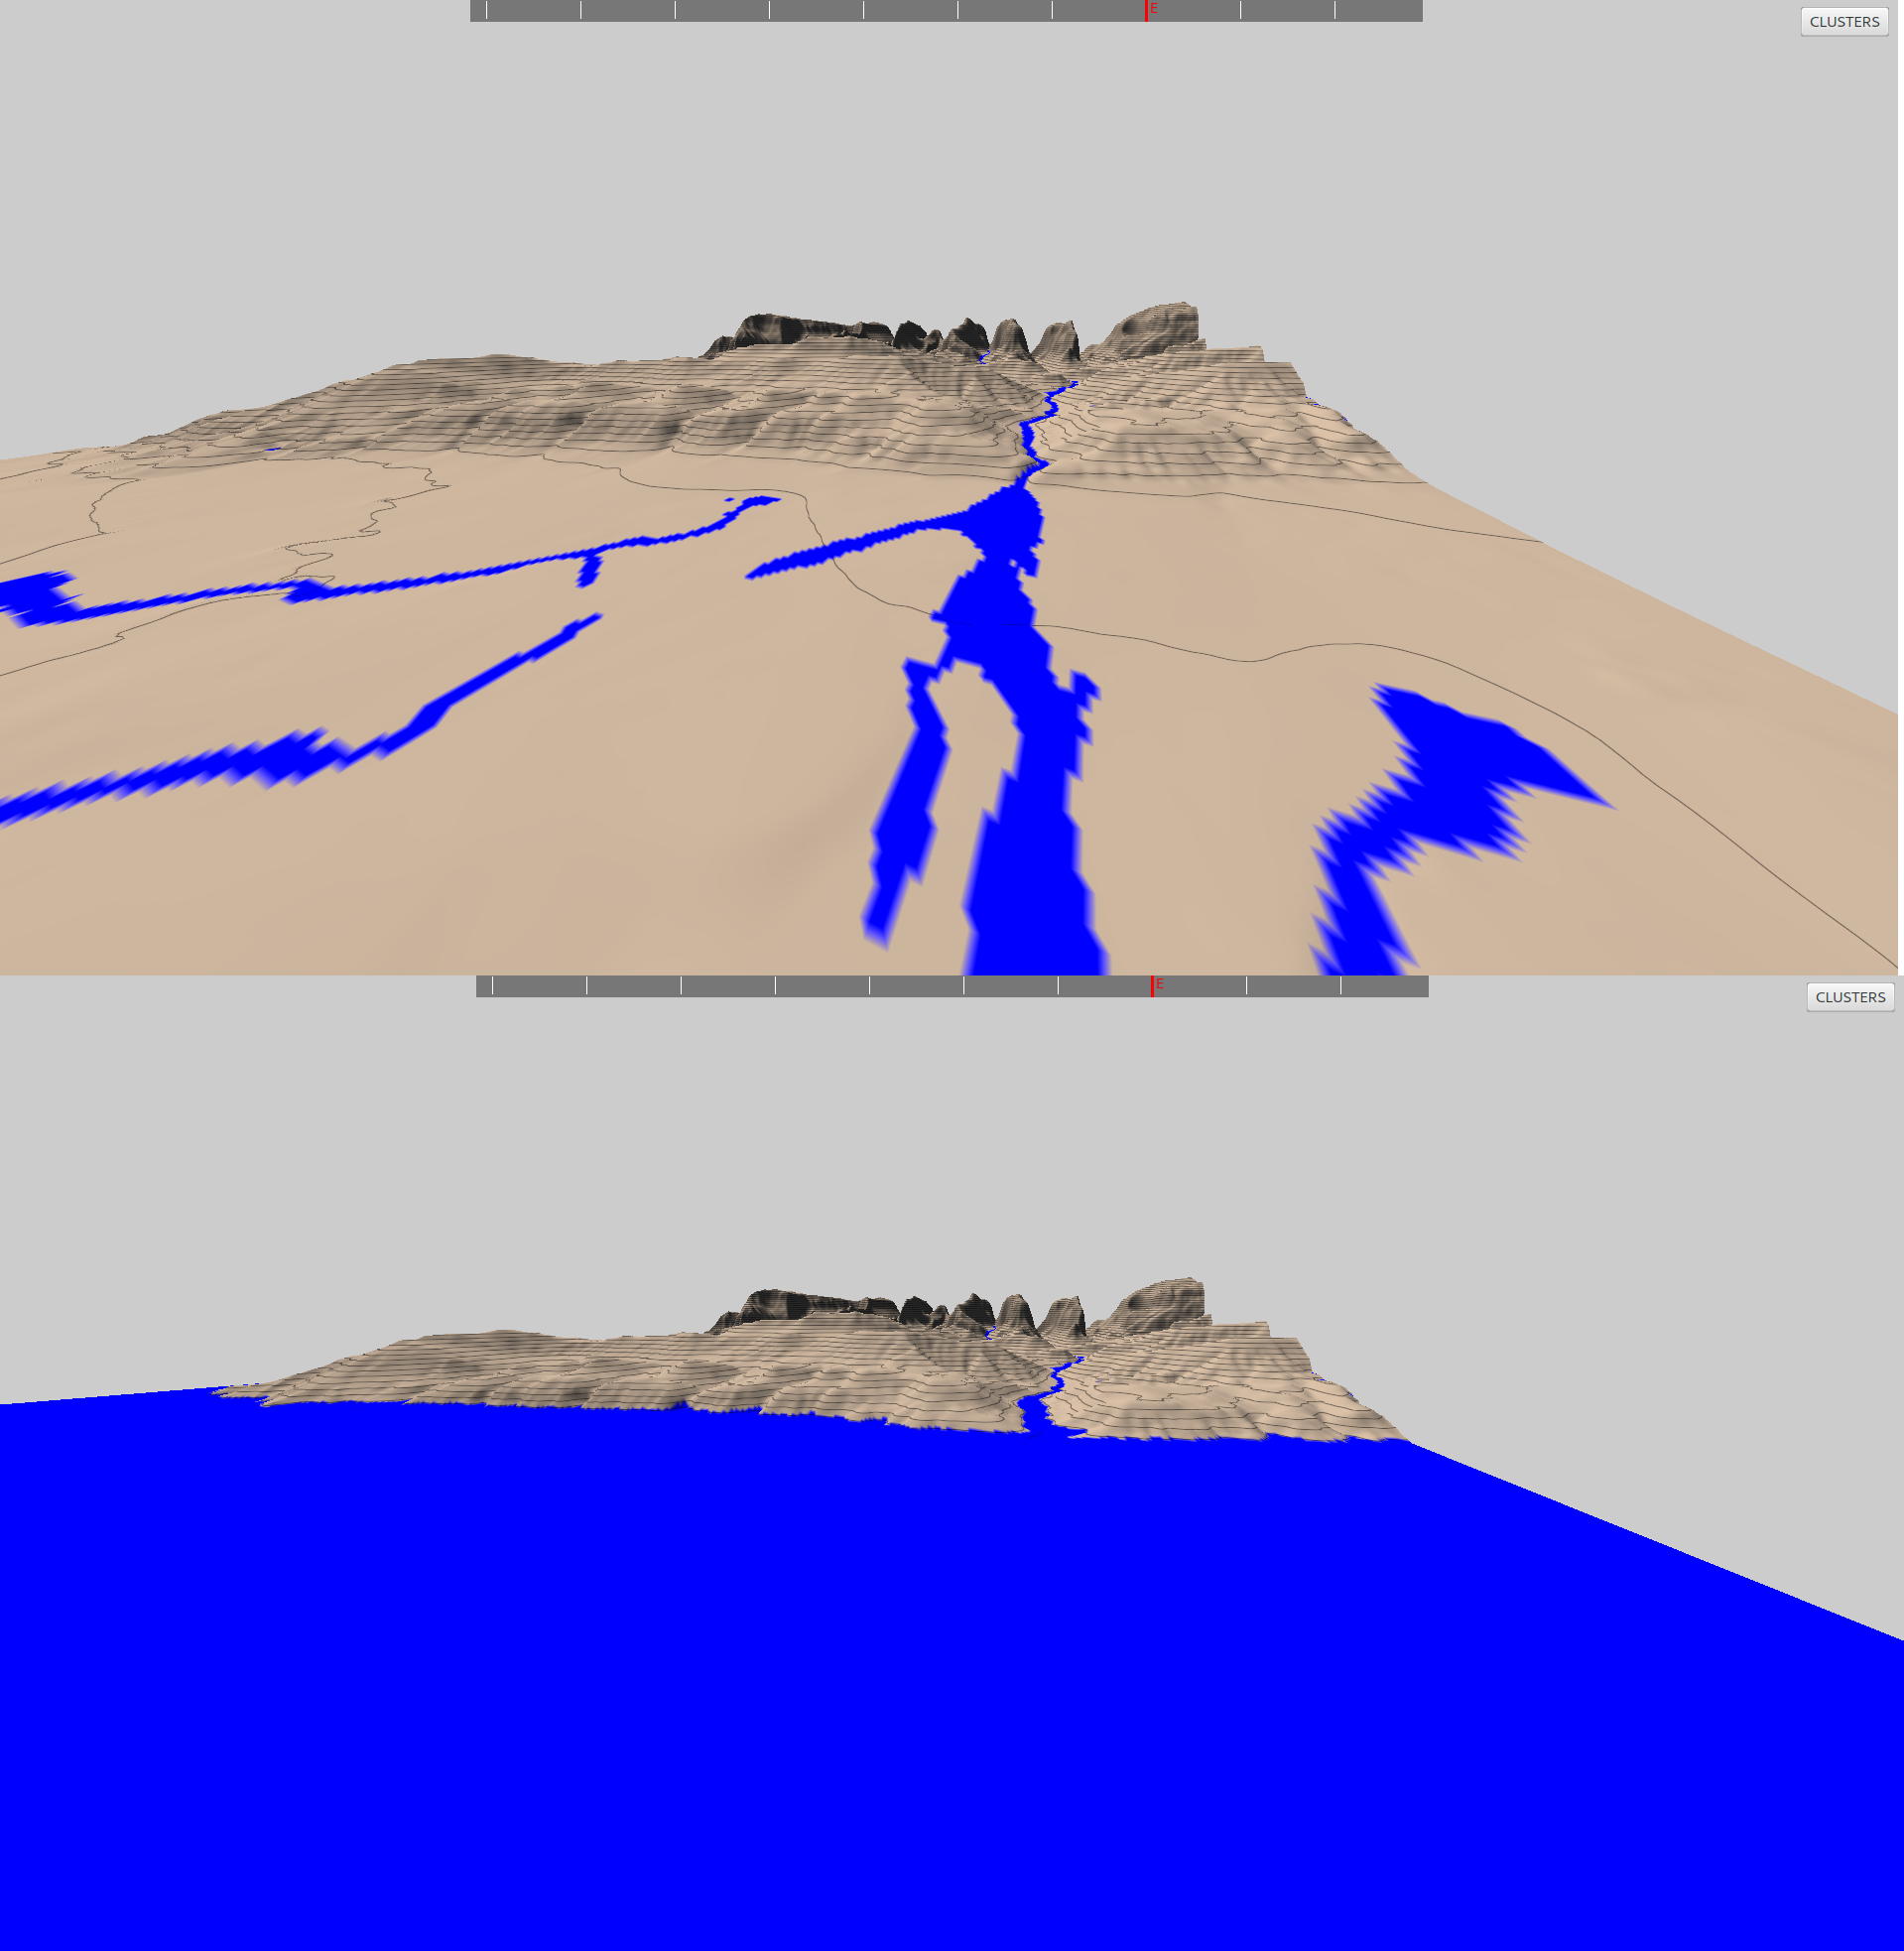
\includegraphics[width=\textwidth]{flood_fill_test_ocean.png}
	\caption{ \textit{Terrain before (top) and after (top) using the flood-fill tool to place a large water body (e.g sea or ocean).} }	
	\label{fig:flood_fill_test}
\end{figure}

\begin{figure}
\center
	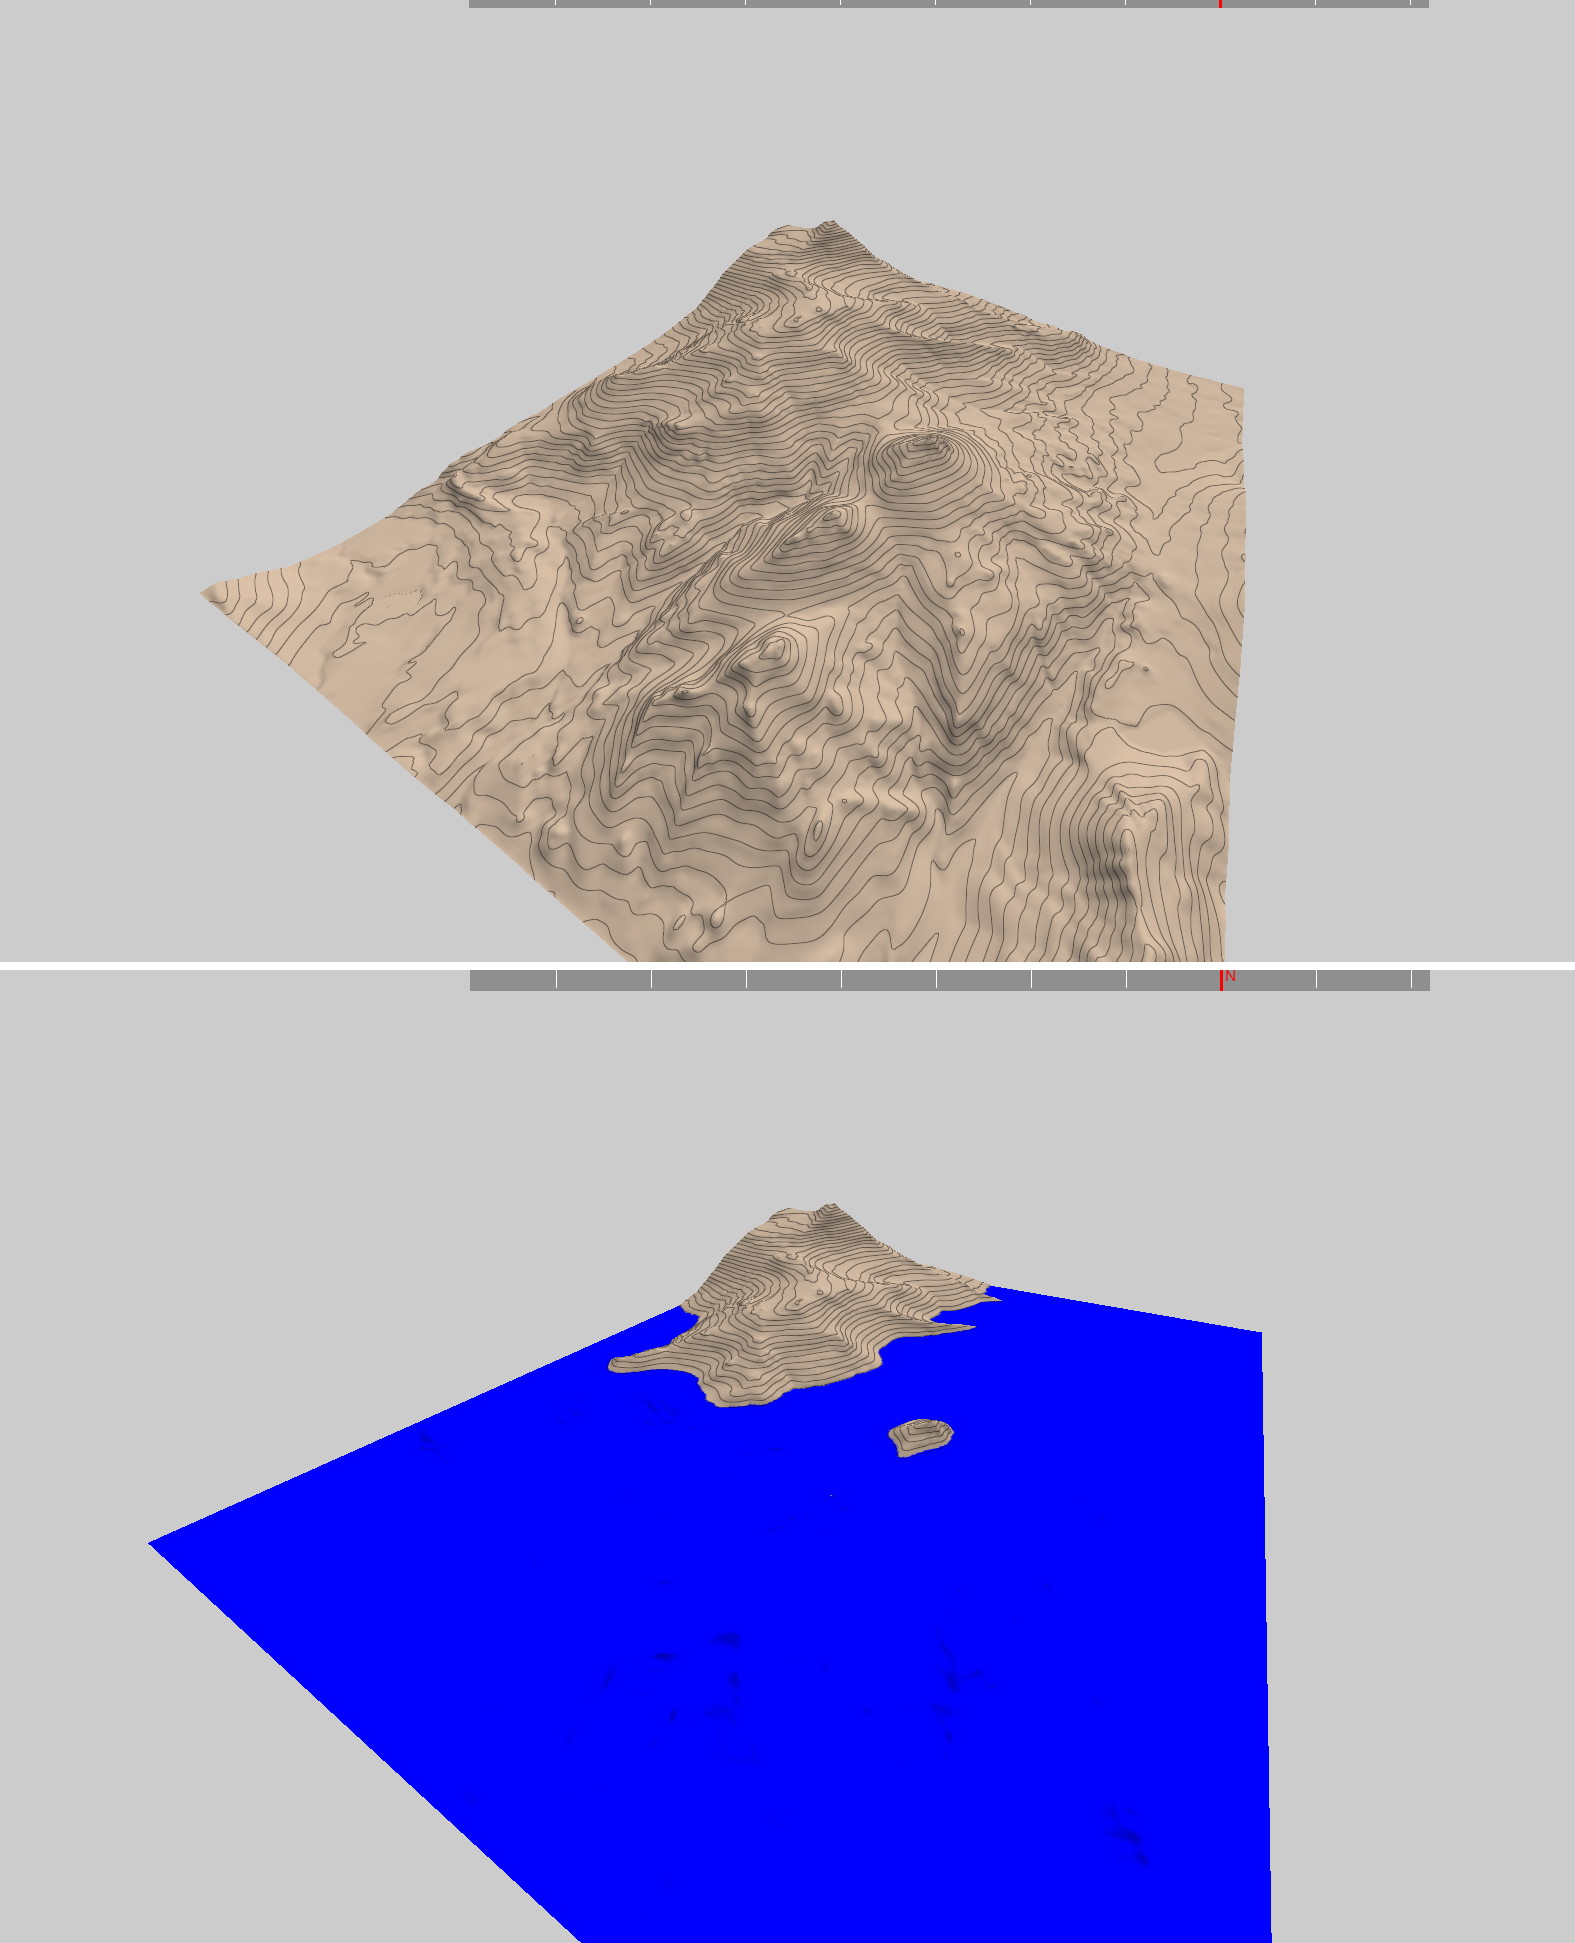
\includegraphics[width=\textwidth]{flood_fill_test_island.png}
	\caption{ \textit{Terrain before (top) and after (top) using the flood-fill tool to place a large water body to make an island.} }	
	\label{fig:flood_fill_test_island}
\end{figure}
